\documentclass[conference]{IEEEtran}
\IEEEoverridecommandlockouts
\usepackage[utf8]{inputenc}
\usepackage[T1]{fontenc}
\usepackage{cite}
\usepackage{amsmath,amssymb}
\usepackage{graphicx}
\usepackage{booktabs}
\usepackage{url}
\usepackage{xcolor}
\usepackage{tikz}
\usetikzlibrary{arrows.meta,positioning}

% generated by research/make_summary.py -- do not edit by hand
\newcommand{\Seeds}{3}
\newcommand{\EmoF}{0.492}
\newcommand{\EmoFsd}{0.002}
\newcommand{\Ekman}{0.617}
\newcommand{\EmoMT}{0.519}
\newcommand{\EmoDistill}{0.490}
\newcommand{\EmoUW}{0.396}
\newcommand{\UWweight}{169.2}
\newcommand{\ValR}{0.707}
\newcommand{\AroR}{0.476}
\newcommand{\ValRcirc}{0.689}
\newcommand{\AroRcirc}{0.382}
\newcommand{\RiskAUROC}{0.995}
\newcommand{\DistF}{0.836}
\newcommand{\STS}{0.830}
\newcommand{\STSmt}{0.643}
\newcommand{\STSteacher}{0.820}
\newcommand{\NRCv}{0.868}
\newcommand{\NRCa}{0.248}
\newcommand{\FaceAcc}{0.516}
\newcommand{\FaceF}{0.494}
\newcommand{\FaceGB}{0.512}
\newcommand{\FaceFACS}{0.375}
\newcommand{\FaceDet}{99.6}
\newcommand{\AgemRecall}{0.95}
\newcommand{\AgemISR}{0.00}
\newcommand{\PlainISR}{0.28}
\newcommand{\PlainRecall}{0.95}
\newcommand{\PlainRedund}{0.67}
\newcommand{\NaiveISR}{0.36}
\newcommand{\ReportRecall}{0.07}
\newcommand{\SafeDevCrisis}{1.00}
\newcommand{\SafeHeldCrisis}{0.90}
\newcommand{\SafeHeldAlert}{1.00}
\newcommand{\SafeVoneHeldCrisis}{0.50}
\newcommand{\SafeClsCrisis}{0.00}
\newcommand{\SafeClsAlert}{0.56}
\newcommand{\SafeLexAlert}{0.94}
\newcommand{\SafeHybAlert}{1.00}
\newcommand{\SafeBenign}{0.04}
\newcommand{\ParityCos}{0.9996}
\newcommand{\ParityTop}{0.990}
\newcommand{\ParityRisk}{0.084}
\newcommand{\SizeQ}{24.2}
\newcommand{\SizeF}{90.5}
\newcommand{\LatQ}{27.8}
\newcommand{\LatF}{4.1}
\newcommand{\AgemThousand}{1.1}
\newcommand{\AgemTenK}{10.3}

\newcommand{\sg}{\operatorname{sg}}

\begin{document}

\title{NeuroCare: Closed-Loop Affective Control for a\\ Private, On-Device Mental-Health Companion}

\author{
\IEEEauthorblockN{Asmit Kundu}
\IEEEauthorblockA{Department of Information Technology\\
Institute of Engineering \& Management, Kolkata, India}
\and
\IEEEauthorblockN{Susovan Jana}
\IEEEauthorblockA{Department of Information Technology\\
Institute of Engineering \& Management, Kolkata, India}
}

\maketitle

\begin{abstract}
Conversational companions for emotional support usually treat emotion as something to display, keep memory as plain retrieval, and rely on the language model itself to behave safely, while sending every sentence to a remote server. We present NeuroCare, a companion that runs entirely on the user's device and uses affect as a control signal. Each turn, a single forward pass of \emph{Aura-Sense}, a 22M-parameter encoder trained jointly for 28-way emotion, valence and arousal, crisis risk and cognitive distortions, yields both the affect reading and the embedding used for memory search. Retrieval-preserving self-distillation keeps that embedding usable (STS-B $\rho$ = \STS, against \STSteacher\ for the frozen encoder and \STSmt\ without distillation), and a circumplex consistency loss learns where each emotion lies on the valence--arousal plane; the learned map agrees with human norms the model never saw (valence $r$ = \NRCv). The reading then drives a three-tier safety gate that can bypass the language model, a router that chooses among six therapeutic stances, and \emph{Affect-Gated Episodic Memory} (AGEM), which recalls relevant memories while keeping painful ones quiet when they are not the topic: on a scripted history it kept recall at \AgemRecall\ while reducing inappropriate resurfacing of painful memories from \PlainISR\ to \AgemISR. A facial channel, \emph{Aura-Face}, classifies expression from 52 blendshape coefficients without ever seeing pixels (\FaceAcc\ accuracy on 8 AffectNet classes). The whole loop runs in a web browser through WebAssembly with outputs verified against the server implementation, or locally with a LoRA fine-tuned Llama~3.2~3B.
\end{abstract}

\begin{IEEEkeywords}
affective computing, mental health, multi-task learning, retrieval-augmented generation, on-device inference, privacy
\end{IEEEkeywords}

\section{Introduction}

Demand for mental-health support far exceeds the supply of professionals \cite{who2022}, and conversational agents have been explored as a first point of contact for people who would otherwise receive nothing \cite{fitzpatrick2017,abdalrazaq2019}. Two obstacles recur. The first is trust: most systems send the user's most private sentences to a remote model. The second is behaviour: a general-purpose language model, even fine-tuned for empathy, does not by itself know when to slow down, when to bring up something said last week, or when to stop generating and point to a human.

NeuroCare began as a local pipeline: a fine-tuned Llama~3.2~3B \cite{grattafiori2024,hu2022lora} served by Ollama, a vector database of past turns, a speech synthesiser and six hand-picked personas. This paper describes how we rebuilt it around a single idea: \emph{affect should be a control signal}, not a decoration. Every turn, the system senses how the person seems to feel, and that reading decides four things: whether the language model is allowed to answer at all, which therapeutic stance it takes, which memories enter its context, and how the session is logged for the person's own reflection.

Our contributions are:
\begin{enumerate}
\item \textbf{Aura-Sense}, a multi-task sentence encoder whose single forward pass serves both memory retrieval and the affect readout. Retrieval-preserving self-distillation prevents task training from destroying the embedding geometry, and a learned circumplex ties discrete emotions to valence and arousal.
\item \textbf{AGEM}, a memory policy that ranks by relevance, emotional salience and recency, gates painful memories by the person's current state, and suppresses immediate repetition.
\item \textbf{A closed affective loop} with a hybrid lexicon--classifier safety gate in front of the language model and an explainable stance router.
\item \textbf{Aura-Face} and a \textbf{zero-server deployment}: facial affect from blendshapes only, and the complete loop running in a browser with verified parity to the server.
\end{enumerate}

\section{Related Work}

\textit{Emotion from text.} GoEmotions \cite{demszky2020} provides 28 fine-grained labels; EmoBank \cite{buechel2017} provides dimensional valence--arousal--dominance ratings. Russell's circumplex \cite{russell1980} links the two views, and the NRC-VAD lexicon \cite{mohammad2018} gives human ratings for emotion words. Most systems predict one view or the other; we learn the mapping between them and validate it against NRC-VAD.

\textit{Multi-task learning and forgetting.} Uncertainty weighting \cite{kendall2018} balances heterogeneous losses. Learning without Forgetting \cite{li2018lwf} and knowledge distillation \cite{hinton2015} preserve a network's earlier behaviour while it learns new tasks. We apply the same principle to the \emph{embedding} of a sentence encoder \cite{reimers2019,wang2020minilm}, so that it keeps serving semantic search \cite{cer2017sts}.

\textit{Memory for language agents.} Retrieval augmentation \cite{lewis2020rag} and agent memory architectures \cite{park2023,packer2023} rank memories by relevance and, in Generative Agents, also by recency and importance \cite{park2023}. None considers that recalling a painful episode can itself cause harm; AGEM adds an affect gate and a refractory period for that reason.

\textit{Safety and clinical language.} Suicide-risk detection from social media \cite{coppersmith2018,komati2021} and cognitive-distortion detection \cite{shreevastava2021,beck1979} are established tasks; the Columbia scale \cite{posner2011} structures ideation severity. We combine a learned risk head with a C-SSRS-organised lexicon and evaluate on short chat messages rather than long posts.

\textit{Facial affect.} AffectNet \cite{mollahosseini2019} is the standard in-the-wild benchmark; FACS \cite{ekman1978} describes expressions as action units. MediaPipe \cite{lugaresi2019,kartynnik2019} estimates 52 blendshape coefficients in real time, which we use as the only input to Aura-Face.

\section{System Overview}

\begin{figure}[t]
\centering
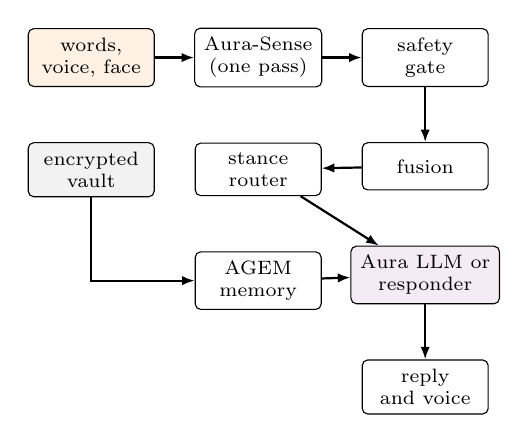
\begin{tikzpicture}[node distance=4mm and 5mm, every node/.style={font=\scriptsize},
  box/.style={draw, rounded corners=2pt, minimum height=6mm, minimum width=16mm, align=center, fill=white},
  arr/.style={-{Latex[length=1.6mm]}, thick}]
\node[box, fill=orange!10] (in) {words,\\voice, face};
\node[box, right=of in] (sense) {Aura-Sense\\(one pass)};
\node[box, right=of sense] (gate) {safety\\gate};
\node[box, below=7mm of gate] (fuse) {fusion};
\node[box, below=7mm of sense] (route) {stance\\router};
\node[box, below=7mm of route] (mem) {AGEM\\memory};
\node[box, below=7mm of fuse, fill=violet!8] (llm) {Aura LLM or\\responder};
\node[box, below=7mm of in, fill=gray!10] (vault) {encrypted\\vault};
\node[box, below=7mm of llm] (out) {reply\\and voice};
\draw[arr] (in) -- (sense);
\draw[arr] (sense) -- (gate);
\draw[arr] (gate) -- (fuse);
\draw[arr] (fuse) -- (route);
\draw[arr] (route) -- (llm);
\draw[arr] (mem) -- (llm);
\draw[arr] (vault) |- (mem);
\draw[arr] (llm) -- (out);
\end{tikzpicture}
\caption{One NeuroCare turn; everything shown runs on the user's device. In a crisis the gate bypasses the language model and returns a fixed message with helplines.}
\label{fig:loop}
\end{figure}

Fig.~\ref{fig:loop} shows one turn. The user's message is read once by Aura-Sense. The safety gate assesses it before any generation. The text reading is fused with optional face and voice cues on the valence--arousal plane, smoothed across turns, and passed to the router, which selects one of six stances: person-centred reflection, grounding, cognitive reframing, behavioural activation, self-compassion or Stoic resilience. AGEM selects memories with the same embedding. The language model, a LoRA fine-tune of Llama~3.2~3B quantised to 4 bits, then streams a reply under the stance's prompt and sampling settings; speech starts after the first sentence. Every stage reports its decision, and the interface shows the person why Aura answered as it did.

Two runtimes implement the loop. The server (Python, FastAPI) uses ONNX Runtime and Ollama and stores memory in SQLite with both text and embeddings sealed by AES-256-GCM, since embeddings can be inverted to recover text \cite{morris2023}. The browser runtime ports every component to JavaScript, runs Aura-Sense through WebAssembly, keeps memory in IndexedDB under a non-extractable WebCrypto key and can load a language model on WebGPU \cite{ruan2024webllm}. A static website therefore offers the complete loop with no server at all.

\section{Aura-Sense}

\subsection{Architecture}
Aura-Sense starts from all-MiniLM-L6-v2 \cite{reimers2019,wang2020minilm}. For input $x$ the encoder $f_\theta$ produces token states, which are mean-pooled and normalised to $e_\theta(x)\in\mathbb{R}^{384}$. Linear heads read $s\,e_\theta(x)$ (with $s=8$): 28 emotion logits $z$, a valence--arousal pair $u=\tanh(\cdot)$, a binary risk head, a binary distortion head and a 10-way distortion-type head. One forward pass returns all of them and the embedding.

\subsection{Retrieval-preserving self-distillation}
Fine-tuning an encoder for classification rotates its embedding space, and the same vector then retrieves poorly. A frozen copy $e_{\theta_0}$ of the original encoder acts as teacher on every batch:
\begin{equation}
\mathcal{L}_{rp} = 1 - \cos\big(e_\theta(x), e_{\theta_0}(x)\big).
\end{equation}

\subsection{Learned circumplex}
A matrix $C\in\mathbb{R}^{28\times2}$, initialised at zero, places each emotion on the valence--arousal plane. With $\hat p = \sigma(z)/\lVert\sigma(z)\rVert_1$ the predicted emotion distribution, $\hat y$ the normalised gold labels and $v$ the EmoBank rating,
\begin{align}
\mathcal{L}_{c1} &= \lVert \hat p\, C - v \rVert^2 \quad \text{(EmoBank batches)},\\
\mathcal{L}_{c2} &= \lVert u - \hat y\, \sg(C) \rVert^2 \quad \text{(GoEmotions batches)}.
\end{align}
$C$ is learned only from dimensional ratings, through the emotion head, and $\mathcal{L}_{c2}$ ties the dimensional head back to the discrete labels. Because NRC-VAD \cite{mohammad2018} is never used in training, the agreement between $C$ and its human norms is an independent check.

\subsection{Objective}
For the four supervised tasks $t$ we use homoscedastic uncertainty weighting \cite{kendall2018}; the consistency term and the distillation term use fixed weights:
\begin{equation}
\mathcal{L} = \sum_t \big(e^{-s_t}\mathcal{L}_t + s_t\big) + \lambda_c(\mathcal{L}_{c1}+\mathcal{L}_{c2}) + \lambda_{rp}\mathcal{L}_{rp}.
\end{equation}
Weighting the consistency term by uncertainty as well proved harmful: its loss is small, so its learned weight grew to \UWweight\ and macro-F1 fell from \EmoDistill\ to \EmoUW\ (Table~\ref{tab:text}).

\subsection{Training}
Each step samples one task with probability proportional to the square root of its training-set size: GoEmotions (43{,}410 sentences, 28 labels \cite{demszky2020}), EmoBank (8{,}062 \cite{buechel2017}), a stratified 30{,}000-post subsample of Reddit posts labelled for suicide risk \cite{komati2021}, and the Shreevastava--Foltz distortion corpus (1{,}720 \cite{shreevastava2021}). We train for 8{,}000 steps (batch 32, AdamW, encoder learning rate $4\times10^{-5}$, mixed precision) on a 4\,GB laptop GPU in about 15 minutes. Thresholds are tuned on validation splits only. The exported graph is quantised to 8-bit block-wise weights with an 8-bit embedding table and fp32 activations: plain dynamic quantisation moved the risk probability by up to 0.65 on some sentences, which we judged unacceptable for a safety signal.

\section{Affect-Gated Episodic Memory}

Each memory $i$ stores an embedding, the valence $v_i$ and arousal $a_i$ read when it was said, its age $\Delta_i$ in days and the turn it last surfaced. For a query with embedding $q$ and current valence $v_q$, with $c_i = q^\top e_i$ and salience $\varsigma_i = \min(1, \lVert(v_i, \max(a_i,0))\rVert)$,
\begin{equation}
\text{score}_i = c_i(1+\beta\varsigma_i) + \gamma\,2^{-\Delta_i/h} - \rho\,\mathbb{1}[\text{surfaced in last } R \text{ turns}].
\end{equation}
A memory is admitted when $c_i \ge \tau$, it is outside the refractory window, and it passes the affect gate: a painful memory ($v_i \le \nu$) is admitted only if the person is low themselves ($v_q \le \nu$) or the query is strongly about it ($c_i \ge \tau_p$). We use $k{=}3$, $\tau{=}0.38$, $\tau_p{=}0.55$, $\nu{=}{-}0.12$, $\beta{=}0.25$, $\gamma{=}0.05$, $h{=}21$, $R{=}3$, $\rho{=}0.6$. Gated candidates are returned with their reason, which the interface shows. Search is exact: at \AgemThousand\,ms for 1{,}000 memories and \AgemTenK\,ms for 10{,}000, an index is unnecessary at personal scale.

\section{Safety, Routing and the Other Senses}

\textit{Safety gate.} Tier~2 (crisis) is raised by explicit ideation, intent, method or self-harm language, or by the risk head above its high-precision threshold together with a distress cue; the language model is then bypassed and a fixed message with regional helplines is shown, and the session stays at tier~1 for four turns. Tier~1 (risk head above its high-recall threshold, or a distress cue) keeps generation but adds a safety instruction. Requests for diagnoses or medication changes add a clinical boundary. The lexicon is organised by C-SSRS categories \cite{posner2011} and is shared verbatim by both runtimes.

\textit{Routing.} The router maps the fused state to a stance with explicit rules: grounding for fear or high-arousal distress, reframing when a distortion is detected on a negative turn, Stoic reflection for anger, self-compassion for signs of depletion, behavioural activation for being stuck, and reflection otherwise. Each stance sets its own temperature and nucleus threshold.

\textit{Aura-Face.} MediaPipe's face landmarker \cite{kartynnik2019} produces 52 blendshape coefficients in the browser. Aura-Face is an ensemble of five two-layer MLPs over a bilateral encoding (unpaired coefficients, then the mean and absolute asymmetry of each of the 20 left--right pairs) trained with mirror augmentation. Its class probabilities are projected through the circumplex $C$ learned by Aura-Sense, so face and text report valence and arousal in one space. Frames never leave the page.

\textit{Voice.} Energy, pitch variability and speaking rate are compared with the user's own running baseline to estimate arousal, which prosody conveys more reliably than valence \cite{scherer2003}.

\textit{Fusion.} Channels are combined per dimension with confidence-weighted priors (text 0.6, face 0.3, voice 0.1 for valence; 0.4, 0.25, 0.35 for arousal) and smoothed across turns, except when the safety tier rises, so that an acute change is never averaged away.

\section{Experiments}

\subsection{Text affect}
Table~\ref{tab:text} compares Aura-Sense with lexical and frozen-encoder baselines, with per-task fine-tuning, and with ablations. Plain multi-task fine-tuning reaches the highest emotion F1 (\EmoMT) but collapses retrieval geometry (STS-B \STSmt). Distillation restores it (\STS, slightly above the frozen encoder's \STSteacher) at a small cost in emotion F1. The circumplex term, with a fixed weight, adds the learned emotion map at no further cost: macro-F1 \EmoF, Ekman macro-F1 \Ekman, crisis-risk AUROC \RiskAUROC, distortion F1 \DistF. Fig.~\ref{fig:ablation} summarises the trade-off and Fig.~\ref{fig:circ} shows the learned map, whose valence coordinates correlate with NRC-VAD at $r$ = \NRCv; arousal agrees less ($r$ = \NRCa), consistent with arousal being the harder dimension in EmoBank itself.

\begin{table*}[t]
\centering
\footnotesize
\caption{Text affect: baselines, ablations and Aura-Sense. Held-out test sets: GoEmotions (5,427), EmoBank (1,000), Reddit risk (10,000), Shreevastava--Foltz (506), STS-B (1,379). For circumplex models, valence and arousal are read through the learned circumplex.}
\label{tab:text}
\setlength{\tabcolsep}{4pt}
\begin{tabular}{lrrrrrrrr}
\toprule
\textbf{Model} & \textbf{Encoder passes / turn} & \textbf{Emotion macro-F1} & \textbf{Ekman macro-F1} & \textbf{Valence r} & \textbf{Arousal r} & \textbf{Risk AUROC} & \textbf{Distortion F1} & \textbf{STS-B $\rho$} \\
\midrule
TF-IDF + logistic / ridge (per task) & -- & 0.443 & 0.564 & 0.509 & 0.271 & 0.980 & 0.826 & -- \\
Frozen MiniLM + task heads & 1 & 0.396 & 0.520 & 0.625 & 0.436 & 0.985 & 0.832 & 0.820 \\
MiniLM fine-tuned separately per task & one per task & 0.435 & 0.600 & -- & -- & 0.996 & -- & -- \\
Multi-task fine-tune & 1 & 0.519 & 0.637 & 0.731 & 0.503 & 0.995 & 0.826 & 0.643 \\
+ retrieval-preserving distillation (n=3 seeds) & 1 & 0.490 $\pm$ 0.002 & 0.612 $\pm$ 0.006 & 0.699 $\pm$ 0.005 & 0.484 $\pm$ 0.009 & 0.995 $\pm$ 0.000 & 0.834 $\pm$ 0.004 & 0.831 $\pm$ 0.001 \\
+ circumplex, uncertainty-weighted & 1 & 0.396 & 0.548 & 0.730 & 0.511 & 0.995 & 0.837 & 0.828 \\
\textbf{Aura-Sense (ours): + circumplex, fixed weight (n=3 seeds)} & \textbf{1} & \textbf{0.492 $\pm$ 0.002} & \textbf{0.617 $\pm$ 0.008} & \textbf{0.689 $\pm$ 0.002} & \textbf{0.382 $\pm$ 0.002} & \textbf{0.995 $\pm$ 0.000} & \textbf{0.836 $\pm$ 0.004} & \textbf{0.830 $\pm$ 0.001} \\
\bottomrule
\end{tabular}
\end{table*}


\begin{figure}[t]
\centering
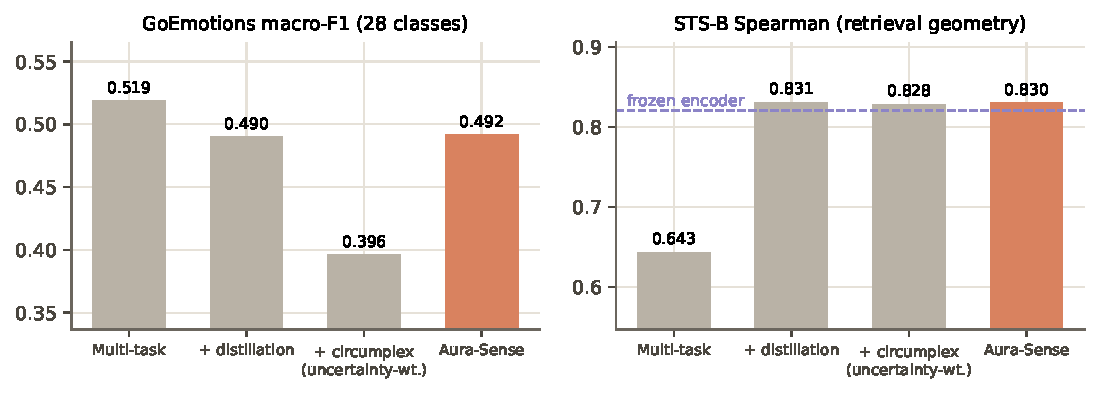
\includegraphics[width=\linewidth]{figures/fig_ablation.pdf}
\caption{Emotion F1 and retrieval quality across the ablation. Distillation is what keeps the shared embedding usable for memory.}
\label{fig:ablation}
\end{figure}

\begin{figure}[t]
\centering
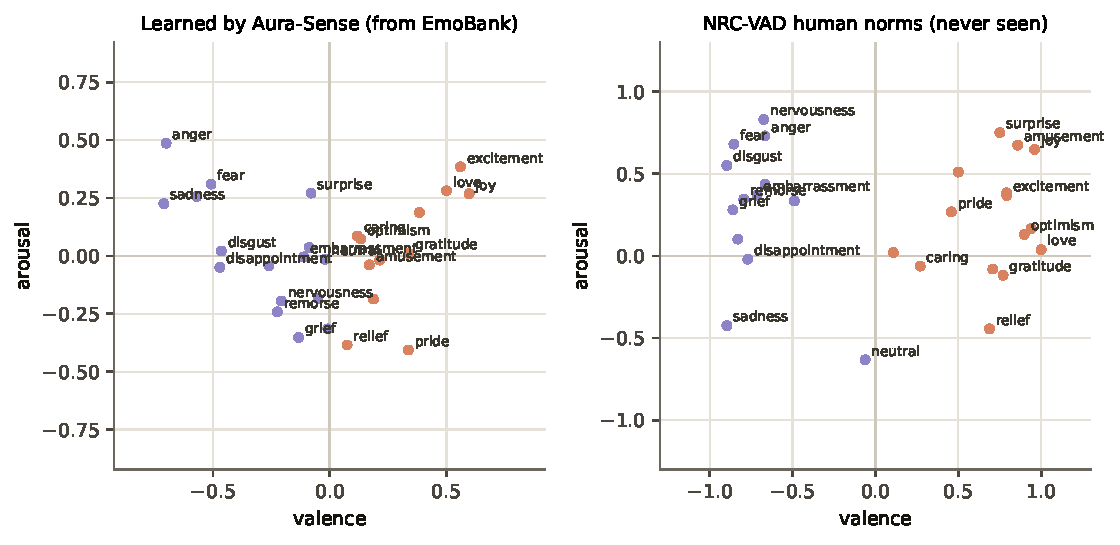
\includegraphics[width=\linewidth]{figures/fig_circumplex.pdf}
\caption{Left: emotion positions learned by Aura-Sense from dimensional ratings alone. Right: human norms from NRC-VAD, never used in training.}
\label{fig:circ}
\end{figure}

\subsection{Memory}
No public benchmark measures whether a companion resurfaces pain at the wrong time, so we scripted a personal history of 20 disclosures, 10 of them painful, and probed it with relevant, unrelated, tangentially related happy, and repeated follow-up queries (Table~\ref{tab:agem}, Fig.~\ref{fig:agem}). The original NeuroCare policy, which always injects the nearest memory, surfaced a painful memory for \NaiveISR\ of unrelated or happy queries. The fixed 0.82 cosine threshold described in our earlier progress report almost never fires with this encoder (recall \ReportRecall). Plain thresholded retrieval recalled well (\PlainRecall) but still surfaced pain at a rate of \PlainISR\ and re-injected the same memory on \PlainRedund\ of follow-up turns. AGEM kept recall at \AgemRecall\ with no inappropriate surfacing and no redundant re-injection; the ablations attribute the first gain to the affect gate and the second to the refractory window. The history is small and author-written, so these figures describe the policy's behaviour rather than population performance.

\begin{table}[t]
\centering
\footnotesize
\caption{Memory policies on a scripted personal history. 20 memories (10 painful), 40 relevant, 15 unrelated and 10 tangential queries, 6 follow-up turns. ISR: share of unrelated or tangential queries where a painful memory was injected (lower is better).}
\label{tab:agem}
\setlength{\tabcolsep}{4pt}
\begin{tabular}{lrrrrr}
\toprule
\textbf{Policy} & \textbf{Recall@3 $\uparrow$} & \textbf{ISR $\downarrow$} & \textbf{Tangential pain $\downarrow$} & \textbf{Silent when unrelated $\uparrow$} & \textbf{Redundancy $\downarrow$} \\
\midrule
naive top-1 (original code) & 1.00 & 0.36 & 0.50 & 0.00 & 0.67 \\
top-3, cos >= 0.82 (progress report) & 0.07 & 0.00 & 0.00 & 1.00 & 0.00 \\
top-3, cos >= 0.38 (plain RAG) & 0.95 & 0.28 & 0.60 & 0.60 & 0.67 \\
AGEM without affect gate & 0.95 & 0.28 & 0.60 & 0.60 & 0.00 \\
AGEM without refractory & 0.95 & 0.00 & 0.00 & 0.60 & 0.50 \\
\textbf{AGEM (full)} & \textbf{0.95} & \textbf{0.00} & \textbf{0.00} & \textbf{0.60} & \textbf{0.00} \\
\bottomrule
\end{tabular}
\end{table}


\begin{figure}[t]
\centering
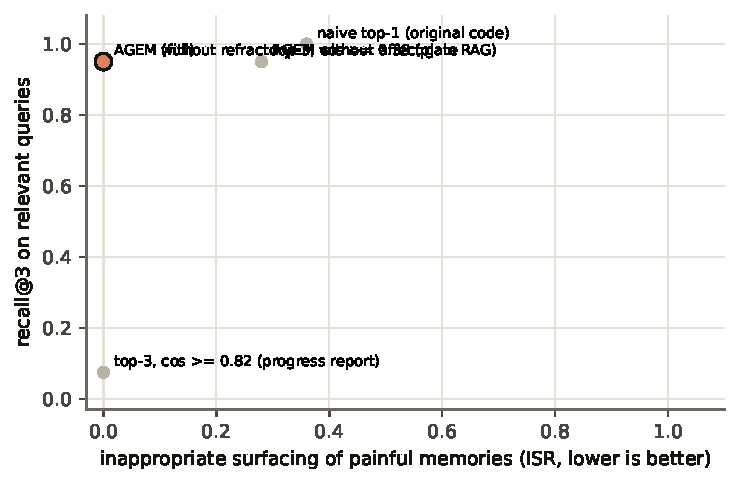
\includegraphics[width=0.92\linewidth]{figures/fig_agem.pdf}
\caption{Recall against inappropriate surfacing of painful memories for each memory policy.}
\label{fig:agem}
\end{figure}

\subsection{Safety}
The risk head separates long posts well (AUROC \RiskAUROC), but a companion receives one-line messages. On a development probe of short messages the classifier alone raised an alert for \SafeClsAlert\ of risk messages and almost never reached the crisis tier, while the lexicon alone reached \SafeLexAlert; the hybrid gate reached \SafeHybAlert\ with a benign false-alert rate of \SafeBenign\ and no over-escalation of ordinary distress (Table~\ref{tab:safety}, Fig.~\ref{fig:safety}). We then wrote a held-out probe, extended the lexicon using development misses only, and re-scored both lexicon versions on the final model: held-out crisis recall rose from \SafeVoneHeldCrisis\ to \SafeHeldCrisis, with alert recall \SafeHeldAlert\ and no false alerts on idioms such as ``this exam is killing me''. Both probes are small and author-written, which makes the held-out estimate optimistic.

\begin{table*}[t]
\centering
\footnotesize
\caption{Safety gate on short conversational messages. Development probe: 20 explicit, 12 indirect, 12 distress, 25 benign. Held-out probe written before lexicon v2: 10 explicit, 8 indirect, 10 idioms. No configuration escalated ordinary distress to a crisis.}
\label{tab:safety}
\setlength{\tabcolsep}{4pt}
\begin{tabular}{lrrrrrr}
\toprule
\textbf{System} & \textbf{Dev crisis recall} & \textbf{Dev alert recall} & \textbf{Dev benign false alert} & \textbf{Held-out crisis recall} & \textbf{Held-out alert recall} & \textbf{Held-out idiom false alert} \\
\midrule
lexicon $\cdot$ lexicon v1 & 0.90 & 0.78 & 0.00 & 0.50 & 0.39 & 0.00 \\
classifier $\cdot$ lexicon v1 & 0.00 & 0.56 & 0.04 & 0.00 & 0.56 & 0.00 \\
hybrid $\cdot$ lexicon v1 & 0.90 & 0.88 & 0.04 & 0.50 & 0.72 & 0.00 \\
lexicon $\cdot$ lexicon v2 & 1.00 & 0.94 & 0.00 & 0.90 & 0.94 & 0.00 \\
classifier $\cdot$ lexicon v2 & 0.00 & 0.56 & 0.04 & 0.00 & 0.56 & 0.00 \\
\textbf{hybrid $\cdot$ lexicon v2} & \textbf{1.00} & \textbf{1.00} & \textbf{0.04} & \textbf{0.90} & \textbf{1.00} & \textbf{0.00} \\
\bottomrule
\end{tabular}
\end{table*}


\begin{figure}[t]
\centering
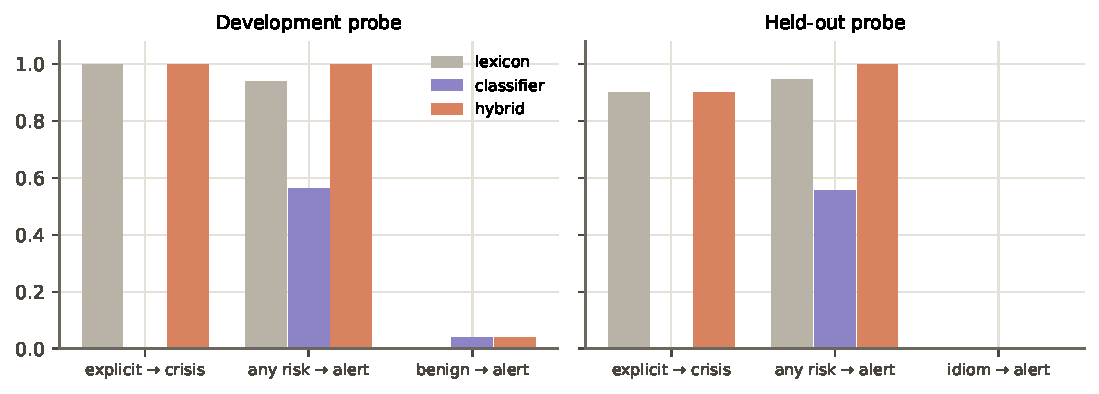
\includegraphics[width=\linewidth]{figures/fig_safety.pdf}
\caption{Lexicon, classifier and hybrid gate on short messages.}
\label{fig:safety}
\end{figure}

\subsection{Facial affect}
Faces were detected in \FaceDet\% of AffectNet test images. Table~\ref{tab:face} shows that blendshapes alone carry substantial signal: zero-shot FACS rules reach \FaceFACS\ accuracy and Aura-Face \FaceAcc\ (macro-F1 \FaceF) across eight classes, on par with gradient boosting (\FaceGB) while running in the browser. The bilateral encoding and mirror augmentation did not improve on a plain MLP by a measurable margin; ensembling did. Pixel-based models score higher on AffectNet, but they see identity and background, which this design rules out by construction.

\begin{table}[t]
\centering
\footnotesize
\caption{Facial affect from blendshapes only (AffectNet, 8 classes). Test n = 5,788, chance accuracy 0.125. Faces detected in 99.6\% of images. No model sees pixels.}
\label{tab:face}
\setlength{\tabcolsep}{4pt}
\begin{tabular}{lrrr}
\toprule
\textbf{Model} & \textbf{Accuracy} & \textbf{Balanced acc.} & \textbf{Macro-F1} \\
\midrule
FACS prototype rules (zero-shot) & 0.375 & 0.316 & 0.279 \\
Logistic regression, 52 coefficients & 0.462 & 0.449 & 0.443 \\
Gradient boosting, 52 coefficients & 0.512 & 0.498 & 0.495 \\
MLP, 52 coefficients & 0.506 & 0.488 & 0.487 \\
MLP + bilateral encoding & 0.507 & 0.483 & 0.487 \\
MLP + mirror augmentation & 0.508 & 0.490 & 0.489 \\
MLP + both & 0.507 & 0.483 & 0.487 \\
\textbf{Aura-Face: 5-member ensemble (deployed)} & \textbf{0.516} & \textbf{0.492} & \textbf{0.494} \\
\bottomrule
\end{tabular}
\end{table}


\subsection{Deployment}
The 8-bit export is \SizeQ\,MB against \SizeF\,MB in fp32 and agrees closely with the PyTorch model (mean embedding cosine \ParityCos, emotion top-1 agreement \ParityTop, largest risk difference \ParityRisk; Table~\ref{tab:runtime}). Block-wise dequantisation makes it slower on a laptop CPU (\LatQ\,ms against \LatF\,ms per sentence at four threads); we accept that cost because it is small next to generation and because the smaller file is what makes free static hosting and quick browser loading practical. A test suite checks that the JavaScript tokenizer produces identical token ids and that the browser runtime reproduces server outputs within $10^{-3}$.

\begin{table*}[t]
\centering
\footnotesize
\caption{Export fidelity and CPU latency of Aura-Sense. Agreement with the PyTorch model on 300 held-out sentences, one sentence per call. Latency is the median per sentence (19.8 tokens on average) on Intel Core i5-11400H (6 cores), 16 GB RAM.}
\label{tab:runtime}
\setlength{\tabcolsep}{4pt}
\begin{tabular}{lrrrrrr}
\toprule
\textbf{Graph} & \textbf{Size (MB)} & \textbf{Embedding cos} & \textbf{Emotion top-1 agree} & \textbf{Max $\Delta$ risk} & \textbf{1 thread (ms)} & \textbf{4 threads (ms)} \\
\midrule
fp32 & 90.5 & 1.0000 & 1.000 & 0.000 & 8.1 & 4.1 \\
\textbf{8-bit weight-only (deployed)} & \textbf{24.2} & \textbf{0.9996} & \textbf{0.990} & \textbf{0.084} & \textbf{47.2} & \textbf{27.8} \\
\bottomrule
\end{tabular}
\end{table*}


\section{Limitations and Ethics}

NeuroCare is a research prototype, not a medical device, and it has not been evaluated with users; a controlled study of perceived empathy, usability and safety is the necessary next step. The risk head is trained on Reddit communities whose labels reflect where a post was made, not clinical assessment. The memory and safety probes are small and author-written. AffectNet labels are themselves noisy, and expression is not emotion. The router's rules encode our reading of the therapeutic literature and should be reviewed by clinicians. A crisis response points to people rather than attempting to manage risk, and the system never diagnoses or advises on medication. All data stay on the user's device, encrypted at rest, and can be exported or erased at any time.

\section{Conclusion}

Treating affect as a control signal turns a local chatbot into a system that decides when to speak, how, and what to remember. A single multi-task encoder makes this cheap enough to run in a browser, retrieval-preserving distillation keeps its embedding useful for memory, and a learned circumplex makes its affect readings interpretable and checkable against human norms. AGEM shows that memory for a companion needs a notion of harm, not only of relevance. The code, models, evaluation scripts and a live demonstration are released with this paper.

\bibliographystyle{IEEEtran}
\bibliography{refs}

\end{document}
